\documentclass{beamer}
\usepackage{beamerthemesplit}
%\usetheme{warsaw}
%\usecolortheme{baylor}
\usetheme[]{utcs}

\usepackage{listings}
%%%%%%%%%%%%%%%%%%%%%%%%%%%%%%%%%%%%%%%%%%%%%%%%%%%%%%%%%%%%%%%%%%%
\usepackage[outdir=./plots/]{epstopdf}
\usepackage{accents}
\usepackage{graphicx}
\usepackage{pgfplots}
\usepackage{pgfplotstable}

% Need this for epstopdf to work correctly.
% This path also needs to not be in the TEXINPUTS path for some reason
\graphicspath{{./../latex-templates/figs/}}

\pgfplotsset{
    discard if not/.style 2 args={
        x filter/.code={
            \edef\tempa{\thisrow{#1}}
            \edef\tempb{#2}
            \ifx\tempa\tempb
            \else
                \def\pgfmathresult{inf}
            \fi
        }
    }
}


\usepackage{minted}

\usepackage{subcaption}
\usepackage{tikz}
\usetikzlibrary{calc}
\usepackage[export]{adjustbox}
%\pagestyle{plain}
%\usepackage{MnSymbol}

\usepackage{amssymb,latexsym,amsmath}
\usepackage{amsfonts}
\usepackage{amsbsy}
\usepackage{color}
\usepackage{multimedia}


\definecolor{red}{rgb}{1.000,0.000,0.000}
\definecolor{green}{rgb}{0.000,0.800,0.200}
\definecolor{blue}{rgb}{0.000,0.300,1.000}
\definecolor{orange}{rgb}{0.800,0.600,0.000}
\definecolor{cyan}{rgb}{0.000,0.600,0.600}
\definecolor{magenta}{rgb}{1.000,0.000,1.000}


\newcommand{\sep}{\setlength\arraycolsep{2pt}}
\def\disp{\displaystyle}

\newcommand{\bfb}{\mathbf{b}}
\newcommand{\bfc}{\mathbf{c}}
\newcommand{\bfx}{\mathbf{x}}
\newcommand{\bfy}{\mathbf{y}}

\newtheorem{proposition}[theorem]{Proposition}
\newtheorem{conjecture}[theorem]{Conjecture}

\newcommand{\la}{\langle}
\newcommand{\ra}{\rangle}
\newcommand{\ketp}{|\psi \rangle}
\newcommand{\brap}{\langle \psi |}
\newcommand{\ketj}{|j \rangle}
\newcommand{\braj}{\langle j |}
\newcommand{\cC}{\mathcal{C}(G,\star)}

\DeclareMathOperator{\Vol}{Vol}
\newcommand{\ria}{\rightarrow}
\newcommand{\riar}{\ria\RR}
\newcommand{\order}[1]{\mathcal{O}\left(#1\right)}

%\newcommand{\range}[1]{\lsem #1 \rsem}
%\newcommand{\comprange}[2]{\lsem #1, #2 \rsem}
%\newcommand{\dimPminus}[3]{\dim P^-_{#1}\Lambda^{#2}(#3)} %r,k,T
%\newcommand{\dimP}[3]{\dim P_{#1}\Lambda^{#2}(#3)} %r,k,T

%\newtheorem{proposition}[theorem]{Proposition}
%\newtheorem{remark}[theorem]{Remark}

\author[BMS]{Robert Kirby$^{1}$
\and Andreas Kl\"ockner$^{2}$
\and Ben Sepanski$^{3}$
}
\date{25 March 2021}
\institute{$^{1}$Baylor University
\\ $^{2}$University of Illinois at Urbana-Champaign
\\ $^{3}$University of Texas at Austin
}
\title{A nonlocal boundary condition for domain truncation in frequency-domain Helmholtz problems}
\logo{
\includegraphics[width=1.5cm]{cslogo.eps}}

\begin{document}
\lstset{language=python}

\frame{\titlepage}

\frame{\tableofcontents}

\frame
{
\frametitle{Thanks to...}
\begin{block}{}
\begin{itemize}
\item NSF 1525697, 1909176
\item The U.S. Department of Energy, Office of
Science, Office of Advanced Scientific Computing
Research, Department of Energy Computational Science
Graduate Fellowship under Award Number DE-SC0021110
\item Luke Olson (UIUC)
\end{itemize}
\end{block}
}

\section{Helmholtz scattering}

\begin{frame}{Model problem}
  \begin{columns}
    \begin{column}{0.45\textwidth}
  \begin{figure}[ht]
    \begin{center}
    \begin{tikzpicture}[scale=0.8]
      \draw [thick,fill=black!30] (-3,-3) rectangle (3,3)
        (0, 0) circle (1);
      \node at (0,0) {$\Omega^c$};
      \node at (-2,2) {$\Omega'$};
      \node [anchor=west] at (1,0) {$\Gamma$};
      \node [anchor=west] at (3,0) {$\Sigma$};
    \end{tikzpicture}
    \end{center}
    %\caption{A 2D example of a truncated domain}
    \label{fig:2ddomain}
  \end{figure}
    \end{column}
    \begin{column}{0.55\textwidth}
      Real problem:
      \[
      \begin{split}
        -\Delta u + \kappa^2 u & = 0,  \ \ \ \mathbb{R}^d \backslash \Omega^c \\
        -\frac{\partial u}{\partial n} & = f, \ \ \ \Gamma \\
            \lim_{r \rightarrow \infty} r^{\tfrac{d-1}{2}} \left(
        \tfrac{\partial u}{\partial r} - i \kappa u
    \right) & = 0,
      \end{split}
      \]
    \end{column}
\end{columns}
\end{frame}

\begin{frame}{Model problem}
  \begin{columns}
    \begin{column}{0.45\textwidth}
  \begin{figure}[ht]
    \begin{center}
    \begin{tikzpicture}[scale=0.8]
      \draw [thick,fill=black!30] (-3,-3) rectangle (3,3)
        (0, 0) circle (1);
      \node at (0,0) {$\Omega^c$};
      \node at (-2,2) {$\Omega'$};
      \node [anchor=west] at (1,0) {$\Gamma$};
      \node [anchor=west] at (3,0) {$\Sigma$};
    \end{tikzpicture}
    \end{center}
    %\caption{A 2D example of a truncated domain}
    \label{fig:pmldomain}
  \end{figure}
    \end{column}
    \begin{column}{0.55\textwidth}
      Computational problem:
      \[
      \begin{split}
        -\Delta u + \kappa^2 u & = 0,  \ \ \ \Omega^\prime \\
        -\frac{\partial u}{\partial n} & =  f, \ \ \ \Gamma \\
        ????? & \ \ \ \Sigma
      \end{split}
      \]
    \end{column}
\end{columns}
\end{frame}

\begin{frame}{Perfectly Matched Layers (PML)}
  \begin{columns}
    \begin{column}{0.5\textwidth}
  \begin{figure}[ht]
    \begin{center}
      \begin{tikzpicture}[scale=0.7]
        \draw [thick,fill=black!60] (-4,-4) rectangle (4,4);
        \draw [thick,fill=black!30] (-3,-3) rectangle (3,3);
        \draw [fill=white] (0, 0) circle (1);
      \node at (0,0) {$\Omega^c$};
      \node at (-2,2) {$\Omega'$};
      \node [anchor=west] at (1,0) {$\Gamma$};
      \node [anchor=west] at (3,0) {$\Omega_S$};
    \end{tikzpicture}
    \end{center}
    %\caption{A 2D example of a truncated domain}
  \end{figure}
    \end{column}
    \begin{column}{0.5\textwidth}
      Computational problem:
      \[
      \begin{split}
        -\nabla \cdot \beta(x) \nabla u + \kappa^2 u & = 0,  \ \ \ \Omega^\prime \\
        -\frac{\partial u}{\partial n} & =  f, \ \ \ \Gamma \\
        u & = 0, \ \ \ \Sigma
      \end{split}
      \]
      \begin{itemize}
      \item<2-> $\beta = I$ in $\Omega^\prime$
      \item<3-> $\beta$ is complex-valued, eats waves in $\Omega_S$
      \item<4-> Solution is right in $\Omega^\prime$
      \item<5-> {\bf Solvers are a pain!}
      \end{itemize}
    \end{column}
\end{columns}  
\end{frame}

\section{A new boundary condition}
\begin{frame}{Integral form of the solution}
With $\mathcal{K}$ the Green's function, the \emph{true} solution satisfies:
  \begin{equation*}
u(x) = \int_\Gamma \left( \tfrac{\partial}{\partial n} \mathcal K(x-y ) \right)u(y) - \left(\tfrac{\partial}{\partial n} u(y) \right) \mathcal K( x - y ) dy,
  \end{equation*}
  where
\visible<2->{
  \begin{equation*}
D(u)(x) = \operatorname{PV} \int_\Gamma \left( \tfrac{\partial}{\partial n} \mathcal K( x-y) \right)u(y) dy, 
\end{equation*}}
\visible<3->{
\begin{equation*}
S(u)(x) = \int  \mathcal K (x - y ) u(y)dy
\end{equation*}
}
\end{frame}

\begin{frame}{Model problem}
  \begin{columns}
    \begin{column}{0.45\textwidth}
  \begin{figure}[ht]
    \begin{center}
    \begin{tikzpicture}[scale=0.8]
      \draw [thick,fill=black!30] (-3,-3) rectangle (3,3)
        (0, 0) circle (1);
      \node at (0,0) {$\Omega^c$};
      \node at (-2,2) {$\Omega'$};
      \node [anchor=west] at (1,0) {$\Gamma$};
      \node [anchor=west] at (3,0) {$\Sigma$};
    \end{tikzpicture}
    \end{center}
    %\caption{A 2D example of a truncated domain}
    %\label{fig:2ddomain}
  \end{figure}
    \end{column}
    \begin{column}{0.55\textwidth}
      \emph{Real} problem
      \[
      \begin{split}
        -\Delta u + \kappa^2 u & = 0,  \ \ \ \Omega^\prime \\
        -\frac{\partial u}{\partial n} & =  f, \ \ \ \Gamma \\
        (i \kappa- \tfrac{\partial}{\partial n})\left( u - D(u) + S(f) \right)& = 0, \ \ \  \Sigma
      \end{split}
      \]
    \end{column}
\end{columns}
\end{frame}

\begin{frame}{Variational form}
  \begin{equation*}
a(u, v) = F(v)
\end{equation*}
for all $v \in H^1(\Omega^\prime)$, \visible<2->{where
\begin{equation*}
a(u, v)
= \left( \nabla u , \nabla v \right) - \kappa^2 \left( u , v \right)
- i \kappa \langle u, v \rangle_{\Sigma}
+ \langle \left( i \kappa - \tfrac{\partial}{\partial n} \right) D(u) , v \rangle_\Sigma
\end{equation*}}%
\visible<3->{and
\begin{equation*}
F(v) = \langle f , v \rangle_\Gamma + \langle\left( i \kappa - \tfrac{\partial}{\partial n} \right) S(f), v \rangle_{\Sigma}
\end{equation*}}
\end{frame}

\begin{frame}{Note}
  \begin{itemize}
  \item<2-> Not DtN (Keller/Givoli): No Fourier series
  \item<3-> Not Poincare-Steklov operator: No singular integrals.
  \end{itemize}
  \visible<4->{
  BUT still requires layer potentials on boundary.}
\end{frame}

\begin{frame}{Theory}
  \begin{itemize}
  \item<2-> $a$ is a bounded bilinear form on $H^1 \times H^1$
  \item<3-> $F$ is a bounded linear functional on $H^1$
  \item<4-> G{\aa}rding inequality.  There exist $M$ and an $\alpha > 0$ such that
\begin{equation*}
\operatorname{Re}(a(u,u)) + M \left\| u \right\|^2 \geq \alpha \left\| u \right\|_{H^1(\Omega)}^2.
\end{equation*}
\item<5-> For $h \leq h_0$, we have optimal-order $H^1$ and $L^2$ error estimates.
  \end{itemize}
\end{frame}

\begin{frame}{Linear system \( A \bfx = \bfb \)}
  Separate out FEM/transmission from layer potential terms:
  \[ A = A^L + A^{NL} \]
  \begin{itemize}
  \item<2-> $A^L$ is built with Firedrake
  \item<3-> $A^{NL}$ is evaluated matrix-free
    \begin{itemize}
    \item<4-> Firedrake -- pytential marshalling
    \item<5-> Pytential constructs layer potential via FMM, evaluates at edge quad points
    \item<6-> Firedrake integrates against test function
    \end{itemize}
  \end{itemize}
\end{frame}

\begin{frame}{Marshalling issue}
  \begin{center}
    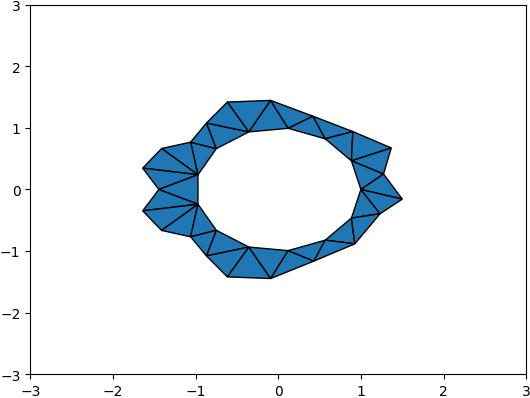
\includegraphics[width=0.7\textwidth]{coarse_near_gamma2d.png}
  \end{center}
\end{frame}

\begin{frame}[fragile]{Numerical results}
\begin{figure}
\begin{center}
    \def \plotaccuracy[#1](#2) % [kappa](color)
    {
        \begin{tikzpicture}[scale=0.5]
        \begin{loglogaxis}[legend style={at={(1.0,0.0)},anchor=south east},
                           xlabel=$h$,
                           ylabel=$L^2$ Error,
                           title={$\kappa=$#1},
                           filter discard warning=false,
                           cycle list={
                               {#2, mark=x}, {#2, mark=o}, {#2, mark=+},
                           },
                           scale=0.8]
            \foreach \method in {pml,transmission,nonlocal} {
                \addplot+[only marks, thick]
                    table [x=h,
                           y expr={\thisrow{kappa}==#1?\thisrow{\method\space lu L2 Error}:nan},
                           col sep=comma] {data/2d_data.csv};
                \addlegendentryexpanded{\method};
            };
        \end{loglogaxis}
        \end{tikzpicture}
        }
    \begin{tabular}{c c}
        \plotaccuracy[0.1](red) & \plotaccuracy[1.0](blue) \\
        \plotaccuracy[5.0](brown) & \plotaccuracy[10.0](black) \\
    \end{tabular}
 \end{center}
\label{fig:2daccuracy}
\end{figure}  
\end{frame}

\begin{frame}{Preconditioning}
  Flexible GMRES requires right-preconditioning:
  \[ A \left( P^{-1} \bfy \right) = \bfb; \ \ \ \bfy = P \bfx \]%
  \visible<2->{Our choice of preconditioner...}
  \visible<3->{
  \[
  P = A^L
  \]}
\end{frame}

\begin{frame}{Using LU on $A^L$}
  \begin{figure}
\begin{center}
\begin{tikzpicture}
    \begin{semilogxaxis}[
        legend style={at={(1.0,0.0)},anchor=south east},
        xlabel=$h$,
        ylabel=Iteration Number,
        filter discard warning=false,
        cycle list={%
            {red, solid, mark=*},
            {blue, densely dotted, mark=square*},
            {brown, densely dashed, mark=triangle*},
            {black, dashdotted, mark=diamond*},
        }]
    \foreach \k in {0.1,1.0,5.0,10.0} {
        \addplot+[thick]
            table [x=h,
                   y expr={\thisrow{kappa}==\k?\thisrow{nonlocal lu Iteration Number}:nan},
                   col sep=comma] {data/2d_data.csv};
       \addlegendentryexpanded{$\kappa=$\k};
    };
    \end{semilogxaxis}
\end{tikzpicture}
\end{center}
\label{fig:luIterationNumber}\end{figure}
\end{frame}

\begin{frame}{Scalable -- gamg?}
\begin{figure}
\begin{center}
\begin{tikzpicture}[scale=0.5]
    \begin{semilogxaxis}[
        legend style={at={(1.0,1.0)},anchor=north east},
        xlabel=$h$,
        ylabel=Iteration Number,
        filter discard warning=false,
        cycle list={%
            {red, solid, mark=*},
            {blue, densely dotted, mark=square*},
            {brown, densely dashed, mark=triangle*},
            {black, dashdotted, mark=diamond*},
        }]
    \foreach \k in {0.1,1.0} {
        \addplot+[thick]
            table [x=h,
                   y expr={\thisrow{kappa}==\k?\thisrow{nonlocal gamg Iteration Number}:nan},
                   col sep=comma] {data/2d_data.csv};
       \addlegendentryexpanded{$\kappa=$\k};
    };
    \end{semilogxaxis}
\end{tikzpicture}
\end{center}
\label{fig:gamgIterationNumber}\end{figure}%
\visible<2->{And explodes for higher $\kappa$.}
\end{frame}

%% \begin{frame}{What about PyAMG (plane waves)?}
%%   \centering
%%   \includegraphics[width=\textwidth]{foo.pdf}
%% \end{frame}
\begin{center}
    \def \plotwcycles[#1]
    {
        \begin{tikzpicture}[scale=0.7]
        \begin{semilogxaxis}[legend style={at={(0.80,0.50)},anchor=south east},
                             xlabel=$h$,
                             ylabel=Iteration Count,
                             title={W-Cycles: #1},
                             filter discard warning=false,
                             cycle list={%
                                {red, solid, mark=*},
                                {blue, densely dotted, mark=square*},
                                {brown, densely dashed, mark=triangle*},
                                {black, dashdotted, mark=diamond*},
                             },
                             scale=0.8]
            \foreach \kappaval in {0.1,1.0,5.0,10.0} {
                \addplot+[thick]
                    table [x=h,
                           discard if not={pyamgmaxiter}{#1},
                            y expr={\thisrow{kappa}==\kappaval?\thisrow{nonlocal pyamg Iteration Number}:nan},
                           col sep=comma] {data/pyamg_2d_data.csv};
                \addlegendentryexpanded{$\kappa=\kappaval$};
            };
        \end{semilogxaxis}
        \end{tikzpicture}
    }
    \begin{tabular}{c c}
        \plotwcycles[1] & \plotwcycles[3]
    \end{tabular}
 \end{center}




\section{Quo vadis, Firedrake? (Future work)}

\begin{frame}[fragile]
  \frametitle{Had NUFL of vaporware?}
  Can we do this?
  \begin{center}
  \begin{minted}[fontsize=\tiny,mathescape]{python}
k = Constant("k")
d = TargetMinusSource(ambient_dim=2)
kernel = ExpressionKernel(
  1/(2*pi)*hankel_1_0(
    k*sqrt(d@d)))

wspace = FunctionSpace(
  Surface(mesh), "Lagrange", 3)
w = Function(wspace)
v = TestFunction(wspace)
bdry_op_sym = inner(
  -0.5*w
  + kernel.conv(w)
  - (source_grad(kernel) 
     @ CellNormal(mesh)
    ).conv(w), v) * dx
\end{minted}
  \end{center}
\end{frame}

\begin{frame}{More generally}
  \begin{itemize}
  \item<2-> Extend UFL with nonlocal operators: Layer/volume potentials, fractional derivatives, etc
  \item<3-> Compiler should segregate local and nonlocal terms:
    \begin{itemize}
    \item<4-> Matrix free, hybrid, HSS, etc
    \item<5-> TSFC + pytential/sumpy/loopy
    \end{itemize}
  \item<6-> Extend solver infrastructure
  \end{itemize}
\end{frame}


\end{document}
